\documentclass[a4paper, 12pt]{article}
\usepackage[T2A,T1]{fontenc}
\usepackage[utf8]{inputenc}
\usepackage[english, russian]{babel}
\usepackage{graphicx}
\usepackage[hcentering, bindingoffset = 10mm, right = 15 mm, left = 15 mm, top=20mm, bottom = 20 mm]{geometry}
\usepackage{multirow}
\usepackage{lipsum}
\usepackage{amsmath, amstext}
\usepackage{siunitx}
\usepackage{subcaption}
\usepackage{wrapfig}
\usepackage{adjustbox}
\usepackage{enumerate, indentfirst, float}
\usepackage{capt-of, svg}

\newenvironment{bottompar}{\par\vspace*{\fill}}{\clearpage}
 
\begin{document}
\begin{titlepage}

\newcommand{\HRule}{\rule{\linewidth}{0.5mm}} % Defines a new command for the horizontal lines, change thickness here

\center % Center everything on the page
 
%----------------------------------------------------------------------------------------
%	HEADING SECTIONS
%----------------------------------------------------------------------------------------

\textsc{\LARGE Московский Физико-Технический Институт}\\[1,5cm] % Name of your university/college
\textsc{\Large Кафедра общей физики}\\[0.5cm] % Major heading such as course name
\textsc{\large Лабораторная работа \textnumero  3.6.1}\\[0.5cm] % Minor heading such as course title

%----------------------------------------------------------------------------------------
%	TITLE SECTION
%----------------------------------------------------------------------------------------

\HRule
\\[0.4cm]
{ \huge \bfseries Спектральный анализ электрических сигналов}
\\[0.2cm] % Title of your document
\HRule
\\[1.5cm]


 
%----------------------------------------------------------------------------------------
%	AUTHOR SECTION
%----------------------------------------------------------------------------------------

\begin{minipage}{0.4\textwidth}
	\begin{flushleft} \large
		\emph{Автор:}\\
		Ришат \textsc{Исхаков} \\
		513 группа
	\end{flushleft}
\end{minipage}
~
\begin{minipage}{0.4\textwidth}
	\begin{flushright} \large
		\emph{Преподаватель:} \\
		Александр Александрович \textsc{Казимиров} % Supervisor's Name
	\end{flushright}
\end{minipage}

\begin{bottompar}
	\begin{center}
		
\includegraphics[width = 80 mm]{logo.jpg}
	\end{center}
	{\large \today}

\end{bottompar}
\vfill % Fill the rest of the page with whitespace

\end{titlepage}

\section{Цель работы}

Изучить спектральный состав периодических электрических сигналов различной формы: последовательности прямоугольных импульсов, последовательности цугов и амплитудно - модулированных гармонических колебаний.

\section{Теоретический материал}

\subsection{Спектральный анализ}

Рассмотрим функцию вида:
$$f(t) = A_{1}cos(\omega_1t-\alpha_{1}) + ... + A_{n}cos(\omega_{n}t-\alpha_{n})$$
или, что то же самое:
$$f(t) = \sum\limits_{i=1}^n A_{i}cos(\omega_{i}t-\alpha_{i})$$
Причем, $A_{i}, \omega_{i}, \alpha_{i}$ - постоянные константы. Множество пар $(\omega_{i}, A_{i}), \: i \in 1..N$ - называется спектром функции $f(t)$.

\subsection{Периодические сигналы}

Часто встречаемая задача - разложение сложного сигнала на гармонические колебания различных частот $\omega$. Представление периодического сигнала в виде суммы гармонических сигналов называется {\it{разложением в ряд Фурье}}.

Пусть заданная функция $f(t)$ - периодически повторяется с частотой $\Omega_{1}=\frac{2\pi}{T}$, где $T$ - период повторения сигнала $f(t)$
Её разложение в ряд Фурье имеет вид:
\begin{equation}
\label{form:furie}	
	f(t)=\frac{a_{0}}{2}+\sum\limits_{n=1}^{\infty}a_{n}\cos(n\Omega_{1}t)+b_{n}\sin(n\Omega_{1}t) 
\end{equation}

или
\begin{equation}
	f(t)=\frac{a_{0}}{2}+\sum\limits_{n=1}^{\infty}A_{n}\cos(n\Omega_{1}t-\psi_{n}) 
\label{form:furie_2}
\end{equation}

где $\frac{a_{0}}{2}$ - среднее значение функции $f(t)$. Постоянные $a_n$ и $b_n$ определяются выражениями:
\begin{equation}
\label{form:a_n}
	a_{n} = \frac{2}{T}\int\limits_{t_{1}}^{t_{1}+T}f(t)\cos(n\Omega_1t)\, dt
\end{equation}

\begin{equation}
	b_{n} = \frac{2}{T}\int\limits_{t_{1}}^{t_{1}+T}f(t)\sin(n\Omega_{1}t)\, dt 
\label{form:b_n}
\end{equation}

причем точку $t_{1}$ можно выбрать любую.

\begin{equation}
\label{form:A_n}
	A_{n} = \sqrt{a_{n}^2+b_{n}^2}
\end{equation}
\begin{equation}
	\psi_{n} = \arctan\frac{b_{n}}{a_{n}}
\label{form:psi_n}
\end{equation}
\section{Работа и измерения}
\subsection*{Исследование спектра периодической последовательности прямоугольных импульсов}

$V_0$  - амплитуда, $\tau$ - длительность, $f_\text{повт} = \frac{2\pi}{T} $ - частота повторения.

Согласно формуле \ref{form:a_n} находим:
$$ \langle V \rangle = \frac{a_0}{2} =  \frac{1}{T}\int\limits_{ -\frac{\tau}{2} } ^ {\frac{\tau}{2} } V_0\,dt = V_0 \frac{\tau}{T}
$$
\begin{equation}
\label{form:app_a_n}
	a_n = \frac{2}{T}\int\limits_{ -\frac{\tau}{2} } ^ {\frac{\tau}{2} } V_0\cos(nf_\text{повт}t)\, dt \sim \frac{\sin(x)}{x}
\end{equation}
 
В силу чётности функции $\forall n \in {N} \ b_n=0$. Таким образом, спектр периодической последовательности прямоугольных импульсов должен выглядеть как график $\frac{\sin(x)}{x}$.
\subsubsection*{Работа}
В работе используются: \textit{анализатор спектра СК4-56; генератор прямоугольных импульсов Г5-54; осциллограф}



\begin{figure}[H]
\centering
\includegraphics[width = 0.8\textwidth]{schemeA}
\caption{Схема для исследования спектра периодической последовательности прямоугольных импульсов}
\label{img:scheme A}
\end{figure}

Собираем схему согласно \ref{img:scheme A}. Получаем на экране осциллографа последовательность периодических прямоугольных импульсов. Подключаем анализатор спектра СК4-56 и после настройки наблюдаем спектр сигнала с параметрами: $$f_\text{повт} = 10^3 \; \text{Гц}, \tau = 25 \; \text{мкс}, m_x = 5 \; \text{кГц}$$

При увеличении частоты повторений $f_\text{повт}$ вдвое при неизменном $\tau$, увеличивается расстояние $\delta \nu$. При увеличении $\tau$ вдвое при неизменной частоте повторений, уменьшается ширина спектра, в соответствии с соотношением неопределенности: $\Delta \nu \tau \simeq 1$.

\subsubsection*{Измерения}
$$\sigma \Delta \nu = 2.5 \; \text{кГц}$$
\begin{table}[H]
\centering
\resizebox{\textwidth}{!}{
\begin{tabular}{|c|c|c|c|c|c|c|c|c|c|c|c|c|c|}
\hline
$\tau, \text{мкс}$   & 25   & 30   & 35   & 40   & 50   & 60   & 70   & 90   & 110 & 130 & 150 & 170 & 200 \\ \hline
$x, \text{клеток}$       & 9    & 7    & 6    & 5    & 4    & 3,3  & 2,9  & 2,3  & 1,8 & 1,5 & 1,5 & 1,2 & 1   \\ \hline
$\Delta \nu, \text{кГц}$ & 45   & 35   & 30   & 25   & 20   & 16,5 & 14,5 & 11,5 & 9   & 7,5 & 7,5 & 6   & 5   \\ \hline
$1/\tau, \text{кГц}$     & 40,0 & 33,3 & 28,6 & 25,0 & 20,0 & 16,7 & 14,3 & 11,1 & 9,1 & 7,7 & 6,7 & 5,9 & 5,0 \\ \hline
\end{tabular}
}
\caption{Зависимость ширины $\Delta \nu$ спектра  от длительности импульса $\tau$}
\end{table}

\begin{figure}[H]
\centering
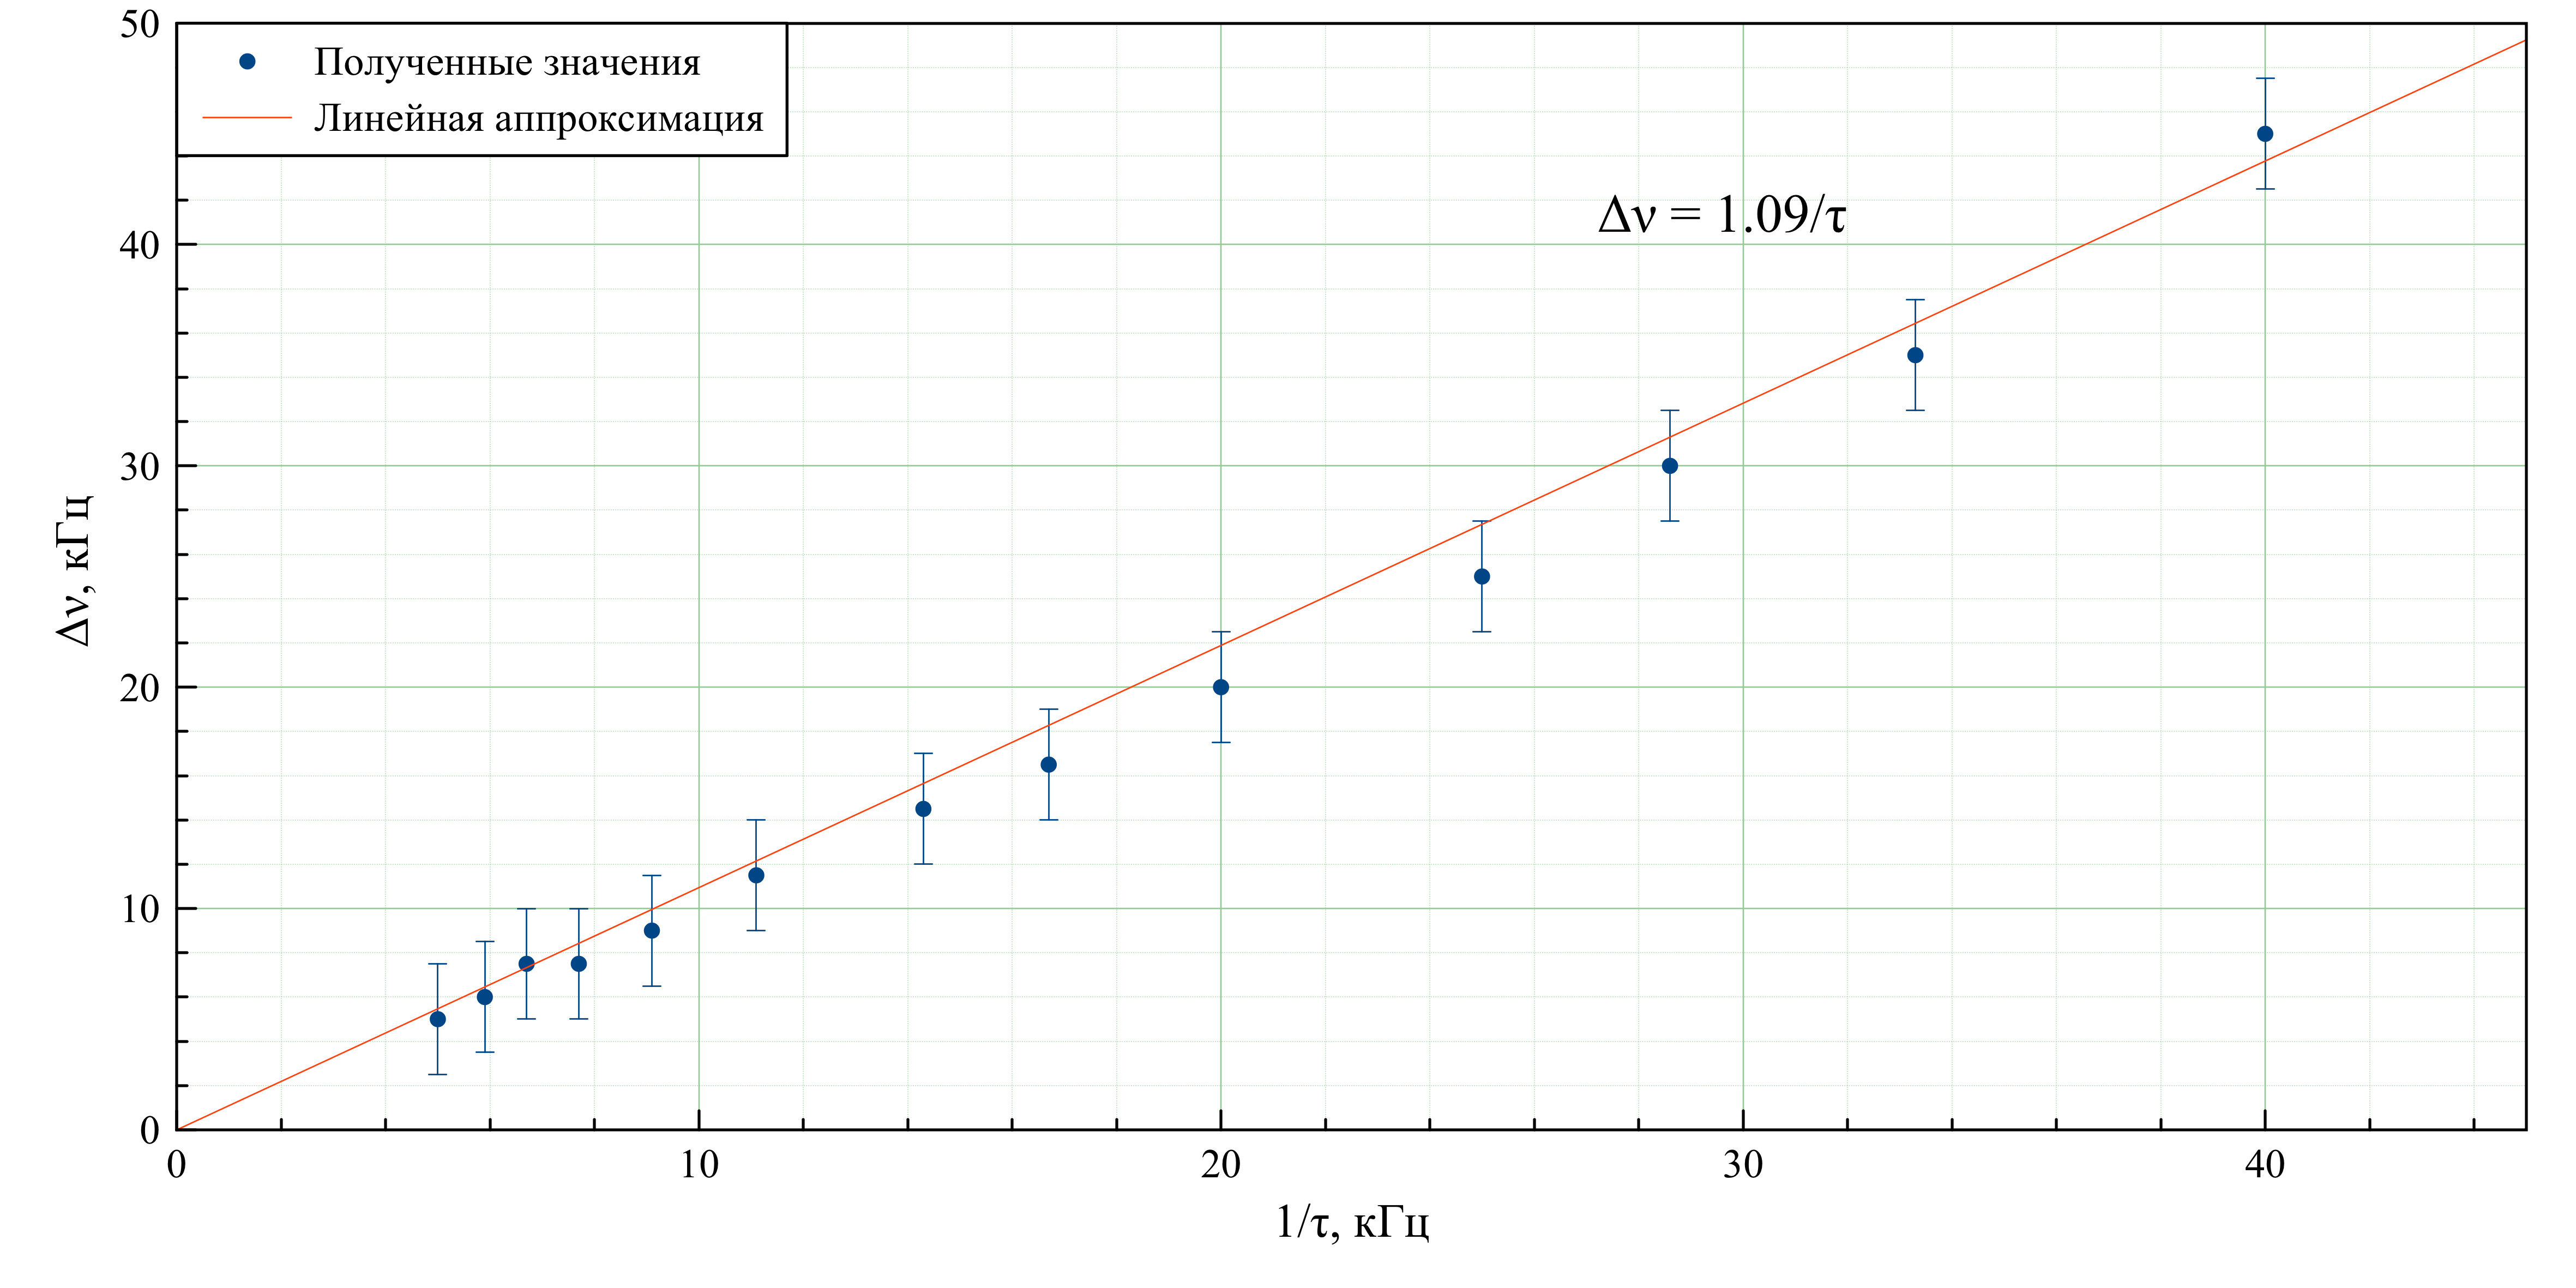
\includegraphics[width = \textwidth]{GraphA}
\caption{График зависимости $\Delta \nu (\frac{1}{\tau})$}
\end{figure}

Коэффициент угла наклона прямой и его погрешность посчитаем методом наименьших квадратов: $k = \langle \Delta \nu \tau \rangle \cdot \langle \tau^2 \rangle$, $\sigma_k = \dfrac{1}{\sqrt{n}} \sqrt{\langle \Delta \nu^2 \rangle \cdot \langle \tau^2 \rangle - k^2}$, тогда $\Delta \nu \tau = 1.1 \pm 0.1$

\begin{figure}[H]
\centering
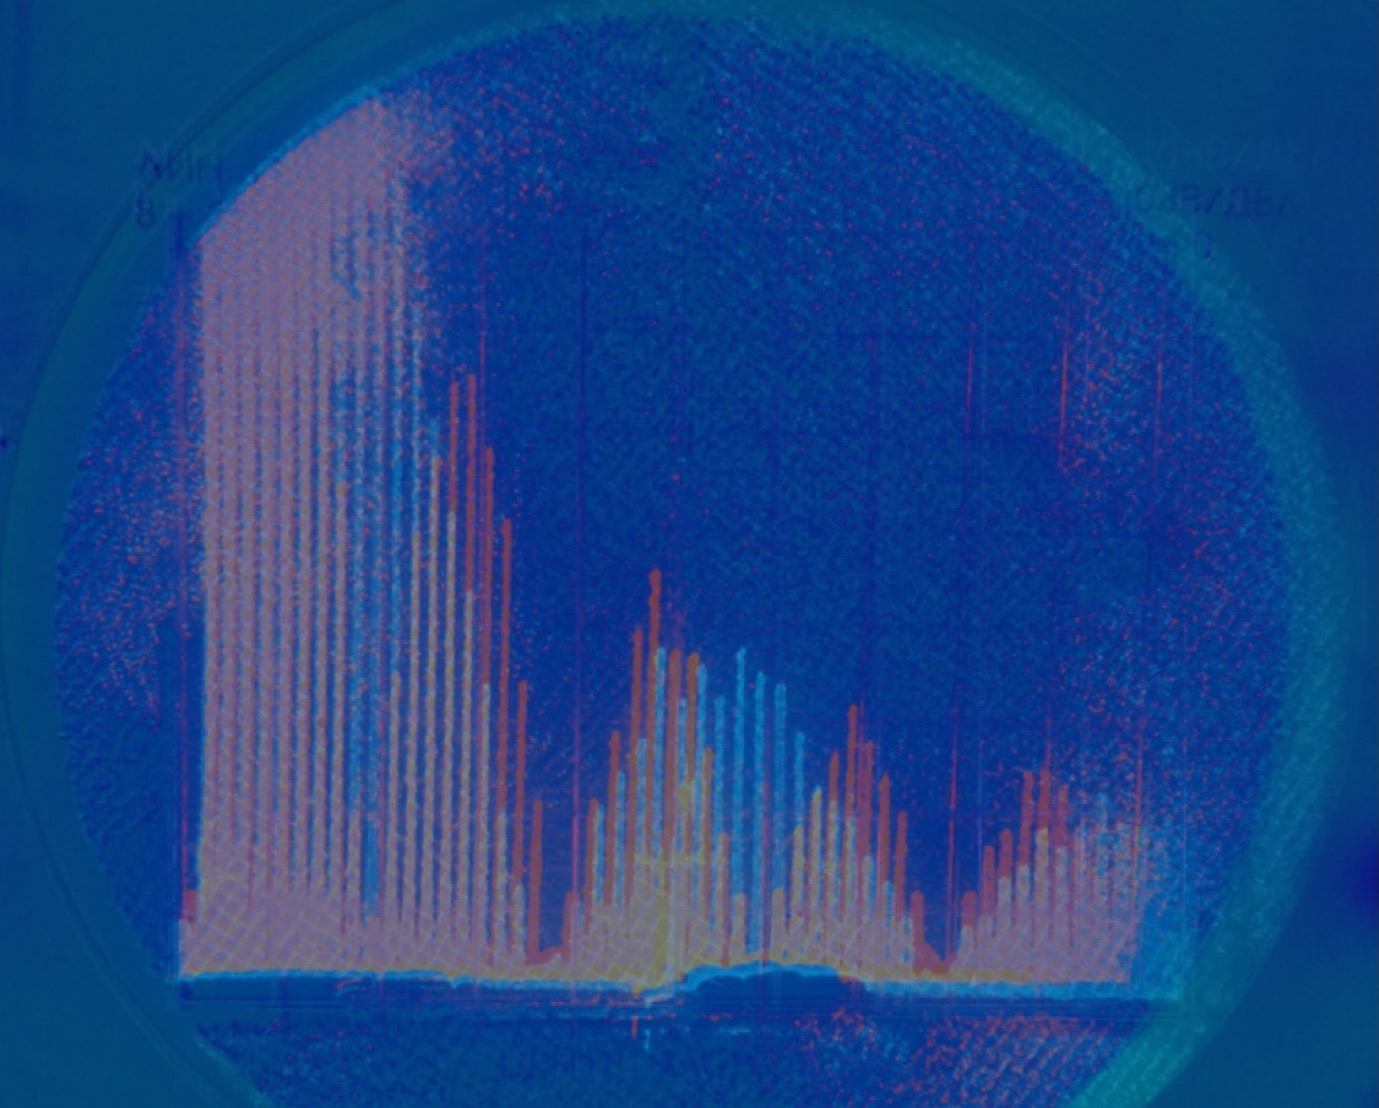
\includegraphics[width = 0.6\textwidth]{A}
\caption{Наложение спектра колебаний с различными параметрами длительности импульса: красный $\tau = 100 \; \text{мкс}$, синий: $\tau = 50 \; \text{мкс}$}
\end{figure}

\subsection*{Исследование спектра периодической последовательности цугов \\ гармонических колебаний}

Рассмотрим периодическую последовательность {\it{цугов}} гармонического колебания \\
$V_0 \cos (\omega_0 t)$ c длительностью цуга $\tau$.
Тогда согласно \ref{form:a_n}:

\begin{equation}
\label{form:cug_a_n}
a_n = \frac{2}{T}\int\limits_{ -\frac{\tau}{2} } ^ {\frac{\tau}{2} } V_0\cos(\omega_0t)\cdot \cos(n\Omega_1)\, dt
\end{equation}

\subsubsection*{Работа}

В работе используются: \textit{анализатор спектра СК4-56; генератор прямоугольных импульсов Г5-54; осциллограф; генератор сигналов Г6-34}

\begin{figure}[H]
\centering
\includegraphics[width = 0.8\textwidth]{schemeB}
\caption{Схема для исследования спектра периодической последовательности цугов высокочастотных колебаний}
\label{img:scheme B}
\end{figure}

Собираем схему согласно \ref{img:scheme B}. Получаем на экране осциллографа последовательность периодических цугов гармонических колебаний, получаемых модулированием синусоиды прямоугольными импульсами. Подключаем анализатор спектра СК4-56 и после настройки наблюдаем спектр сигнала с параметрами: $$ \nu_0 = 25 \; \text{кГц}, f_\text{повт} = 10^3 \; \text{Гц}, \tau = 100 \; \text{мкс}, m_x = 5 \; \text{кГц}$$

При увеличении $\tau$ вдвое при неизменной частоте повторений, вдвое уменьшается ширина спектра, в соответствии с соотношением неопределенности: $\Delta \nu \tau \simeq 1$.

При изменении несущей частоты  $\nu_0 = 25, 10 \; \text{или} \; 40\; \text{кГц}$ при неизменных $f_\text{повт} = 10^3 \; \text{Гц}, \tau = 100 \; \text{мкс}, m_x = 5 \; \text{кГц}$, изменяется сдвиг спектра по оси частот.

\begin{table}[H]
\centering
\begin{tabular}{|c|c|c|c|c|c|c|c|c|}
\hline
$f_\text{повт}, \text{кГц}$ & 1    & 2    & 3    & 4    & 5    & 6    & 7    & 8    \\ \hline
$x, \text{клеток}$          & 3    & 3    & 3    & 3    & 3    & 10   & 10   & 10   \\ \hline
$n, \text{штук}$                        & 16   & 8    & 6    & 4    & 3    & 9    & 7,5  & 7    \\ \hline
$\delta \nu, \text{кГц}$    & 0,94 & 1,88 & 2,50 & 3,75 & 5,00 & 5,56 & 6,67 & 7,14 \\ \hline
$\sigma \delta \nu$      & 0,12 & 0,47 & 0,83 & 0,94 & 0,83 & 0,62 & 0,89 & 1,02 \\ \hline
\end{tabular}
\caption{Зависимость расстояния между соседними спектральными компонентами от $f_\text{повт}$ при $\tau = 50 \text{мкс}$ }
\end{table}

\begin{figure}[H]
\centering
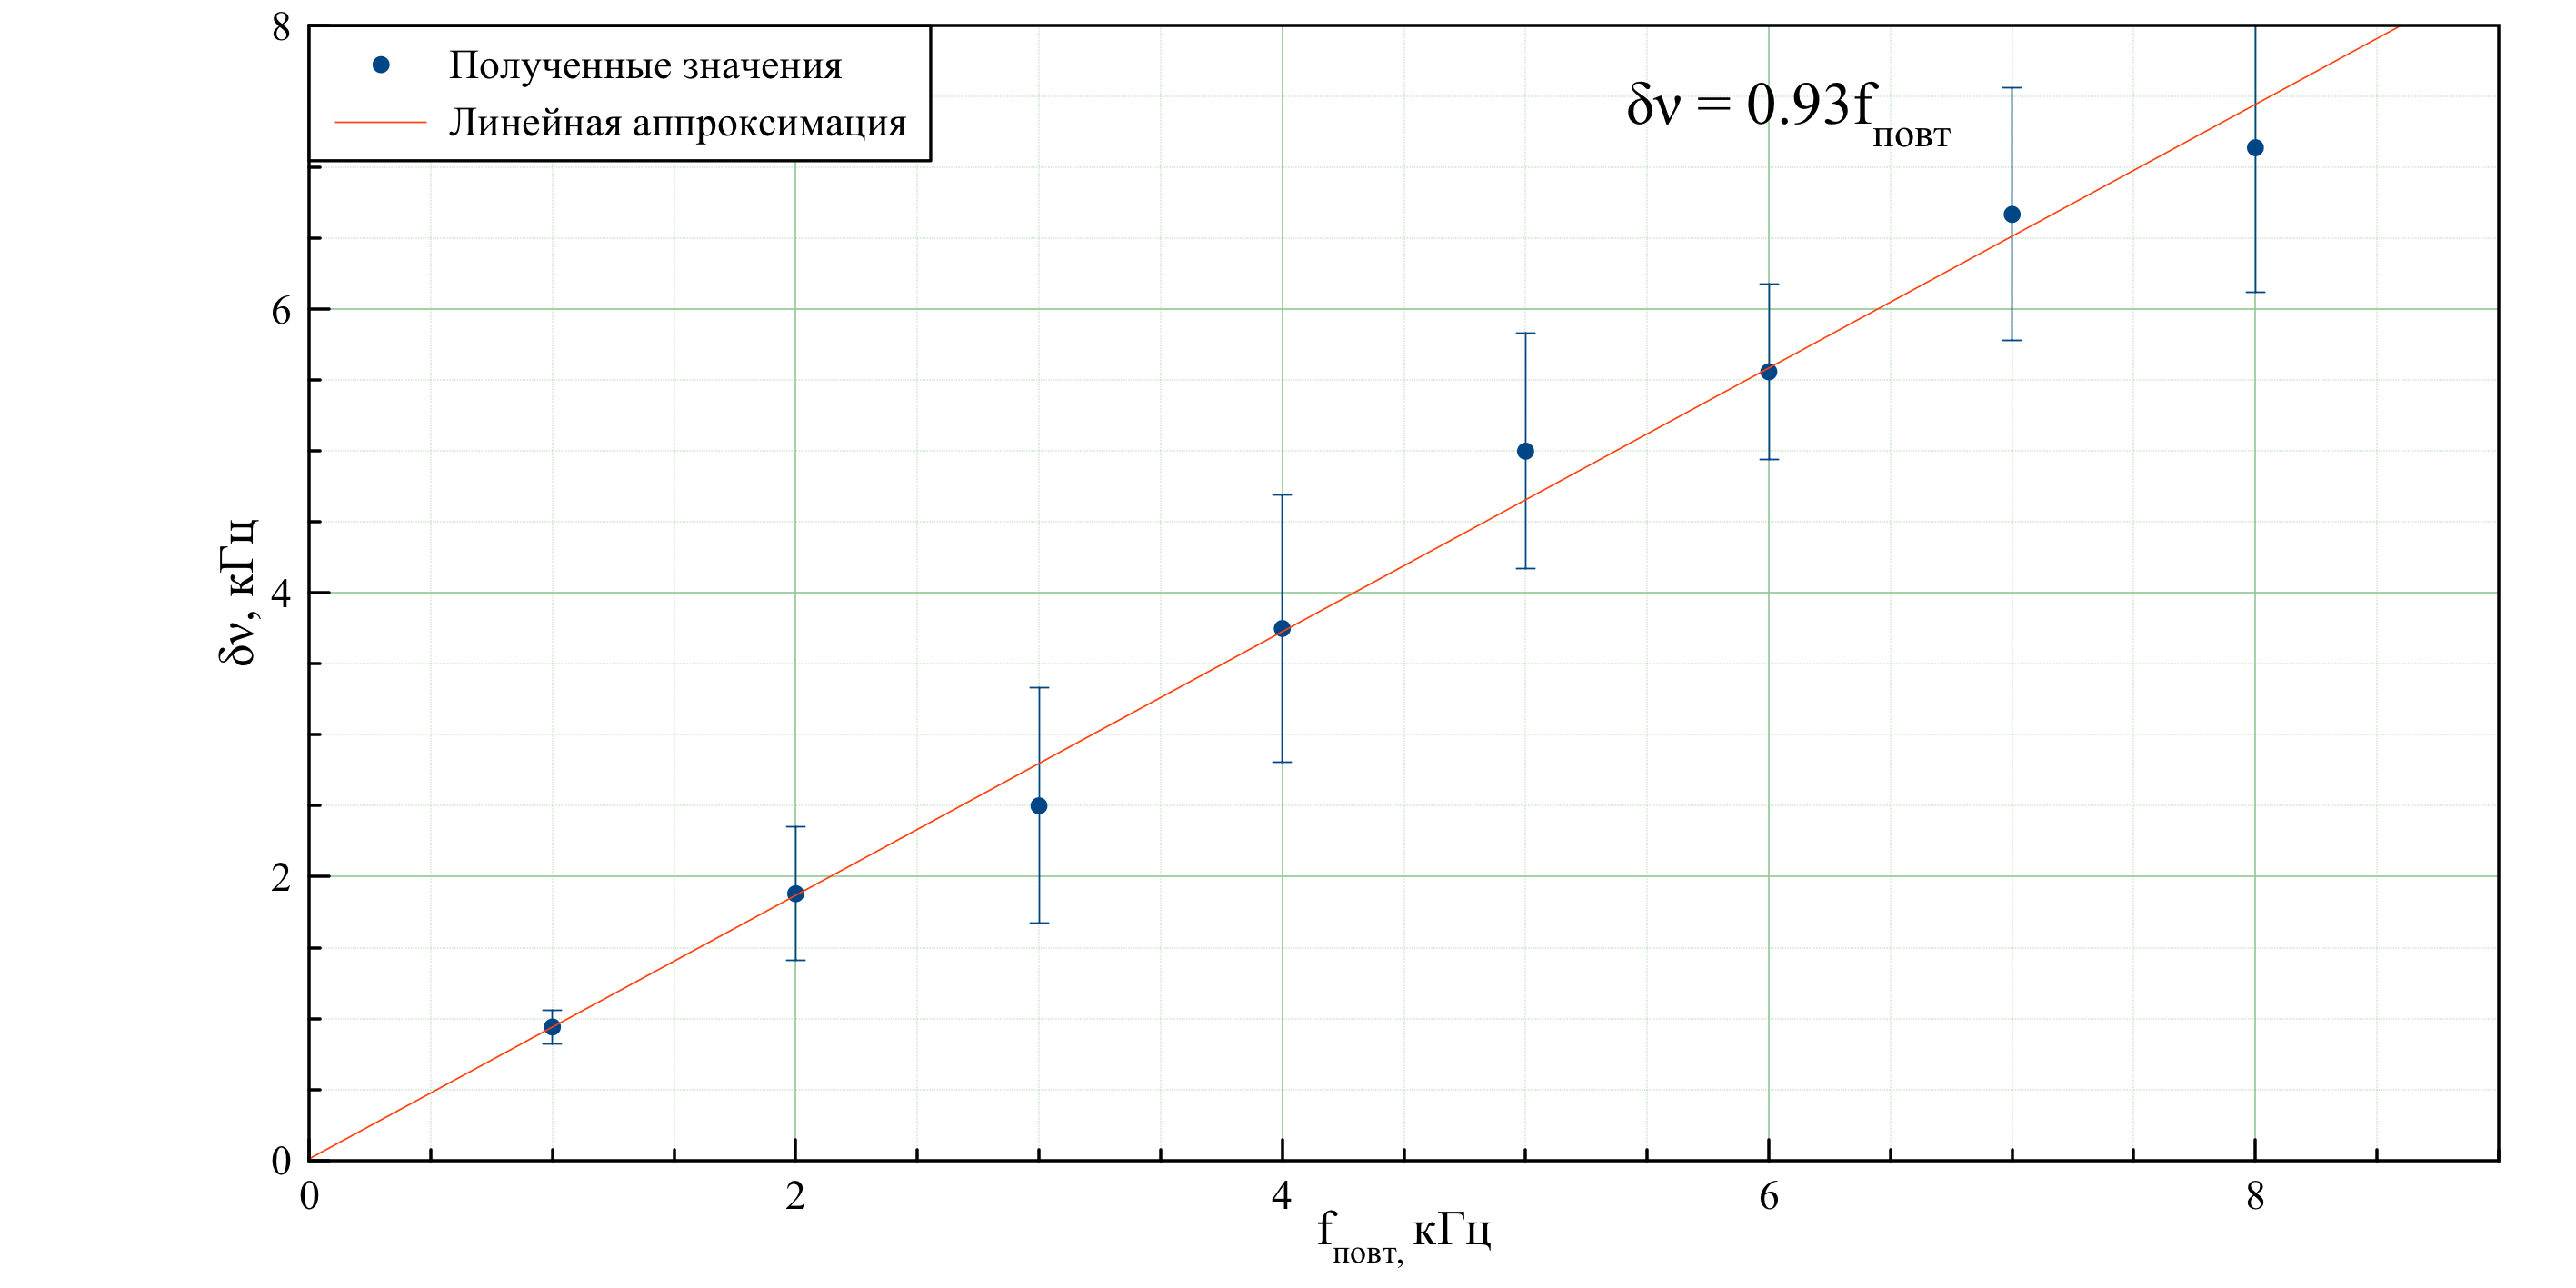
\includegraphics[width = \textwidth]{GraphB}
\caption{График зависимости $\delta \nu (f_\text{повт})$}
\end{figure}

Коэффициент угла наклона прямой и его погрешность посчитаем методом наименьших квадратов: $k = \dfrac{\langle \delta \nu f_\text{повт}  \rangle}{\langle f_\text{повт}^2 \rangle}$, $\sigma_k = \dfrac{1}{\sqrt{n}} \sqrt{\dfrac{\langle \delta \nu^2 \rangle}{\langle f_\text{повт}^2 \rangle} - k^2}$, тогда $\Delta \nu \tau = 0.93 \pm 0.17$

\begin{figure}[H]
\centering
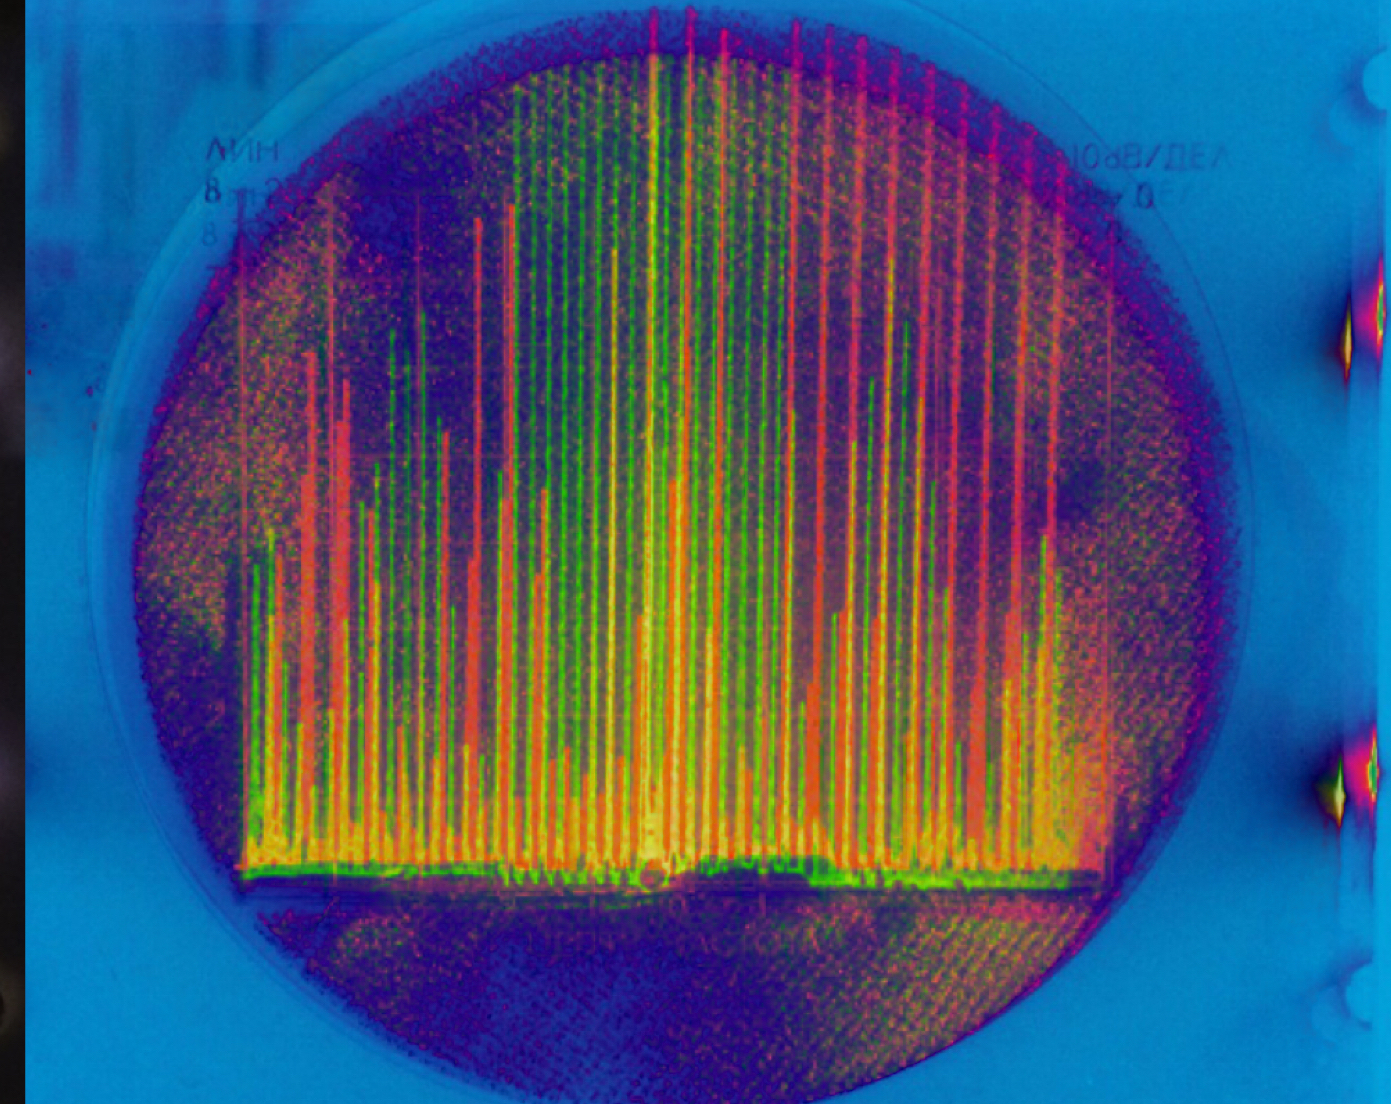
\includegraphics[width = 0.6\textwidth]{B}
\caption{Наложение спектра колебаний с различными частотами повторения: синий: $f_\text{повт} = 1 \text{кГц}$, красный: $f_\text{повт} = 2 \text{кГц}$}
\end{figure}

\subsection*{Исследование спектра гармонических сигналов, модулированных по амплитуде}

Рассмотрим гармонические колебания высокой частоты $\omega_0$, амплитуда которых, в свою очередь, меняется по гармоническому закону с частотой $\Omega \ll \omega_0$.

\begin{equation}
\label{form:amf(t)_a_n}
	f(t) = A_0[1+m\cos(\Omega t)]\cos(\omega_0t)
\end{equation}

Коэффициент $m$ - глубина модуляции и по определению:
\begin{equation}
\label{form:m}
	m = \frac{A_{max}-A_{min}}{A_{max}+A_{min}}
\end{equation}

\subsubsection*{Работа}
В работе используются: \textit{анализатор спектра СК4-56; генератор прямоугольных импульсов Г5-54; осциллограф; генератор сигналов Г6-34}

\begin{figure}[H]
\centering
\includegraphics[width = 0.8\textwidth]{schemeC}
\caption{Схема для исследования спектра гармонических сигналов, модулированных по амплитуде}
\label{img:scheme C}
\end{figure}

Собираем схему согласно \ref{img:scheme C}. Получаем на экране осциллографа гармонический сигнал, модулированный по амплитуде. Подключаем анализатор спектра СК4-56 и после настройки наблюдаем спектр сигнала.

Чтобы измерить глубину модуляции, измерим $A_{max}$, $A_{min}$ и подставим в формулу \ref{form:m}. Построим график отношения $a_\text{бок}/a_\text{осн}$ в зависимости от $m$.

Рассчитаем теоретический коэффициент наклона, воспользовавшись формулой:
\begin{equation}
\label{form:a/a(m)}
	f(t)=A_0\cos(\omega_0t)+	\frac{A_0m}{2}\cos(\omega_0+\Omega t)+\frac{A_0m}{2}\cos(\omega_0-\Omega t). 
\end{equation}

$$a_\text{осн} = A_0, \; a_\text{бок}= \frac{A_0m}{2} \Rightarrow k_\text{теор} = =0.5$$
	
\begin{table}[H]
\centering
\caption{Зависимость отношения амплитуды боковой линии спектра к амплитуде основной линии $a_\text{бок}/a_\text{осн}$ от глубины модуляции $m$}
\begin{tabular}{|c|c|c|c|c|c|c|}
\hline
$2A_{min}, \text{мм}$ & $2A_{max}, \text{мм}$ & $m$  & $a_\text{бок}, \text{мм}$ & $a_\text{осн}, \text{мм}$ & $a_\text{бок}/a_\text{осн}$ & $\sigma_{a_\text{бок}/a_\text{осн}}$ \\ \hline
0,80                & 6,50                & 0,78 & 2,20                      & 6,20                      & 0,35                        & 0,02                               \\ \hline
2,70                & 4,40                & 0,24 & 0,60                      & 6,70                      & 0,09                        & 0,01                               \\ \hline
1,60                & 5,70                & 0,56 & 1,90                      & 6,30                      & 0,30                        & 0,02                               \\ \hline
1,20                & 6,20                & 0,68 & 2,40                      & 6,50                      & 0,37                        & 0,02                               \\ \hline
0,80                & 6,60                & 0,78 & 2,50                      & 6,40                      & 0,39                        & 0,02                               \\ \hline
0,40                & 7,00                & 0,89 & 3,00                      & 6,50                      & 0,46                        & 0,02                               \\ \hline
0,20                & 7,20                & 0,95 & 3,10                      & 6,40                      & 0,48                        & 0,02                               \\ \hline
2,20                & 5,00                & 0,39 & 1,20                      & 6,40                      & 0,19                        & 0,02                               \\ \hline
\end{tabular}
\end{table}

\begin{figure}[H]
\centering
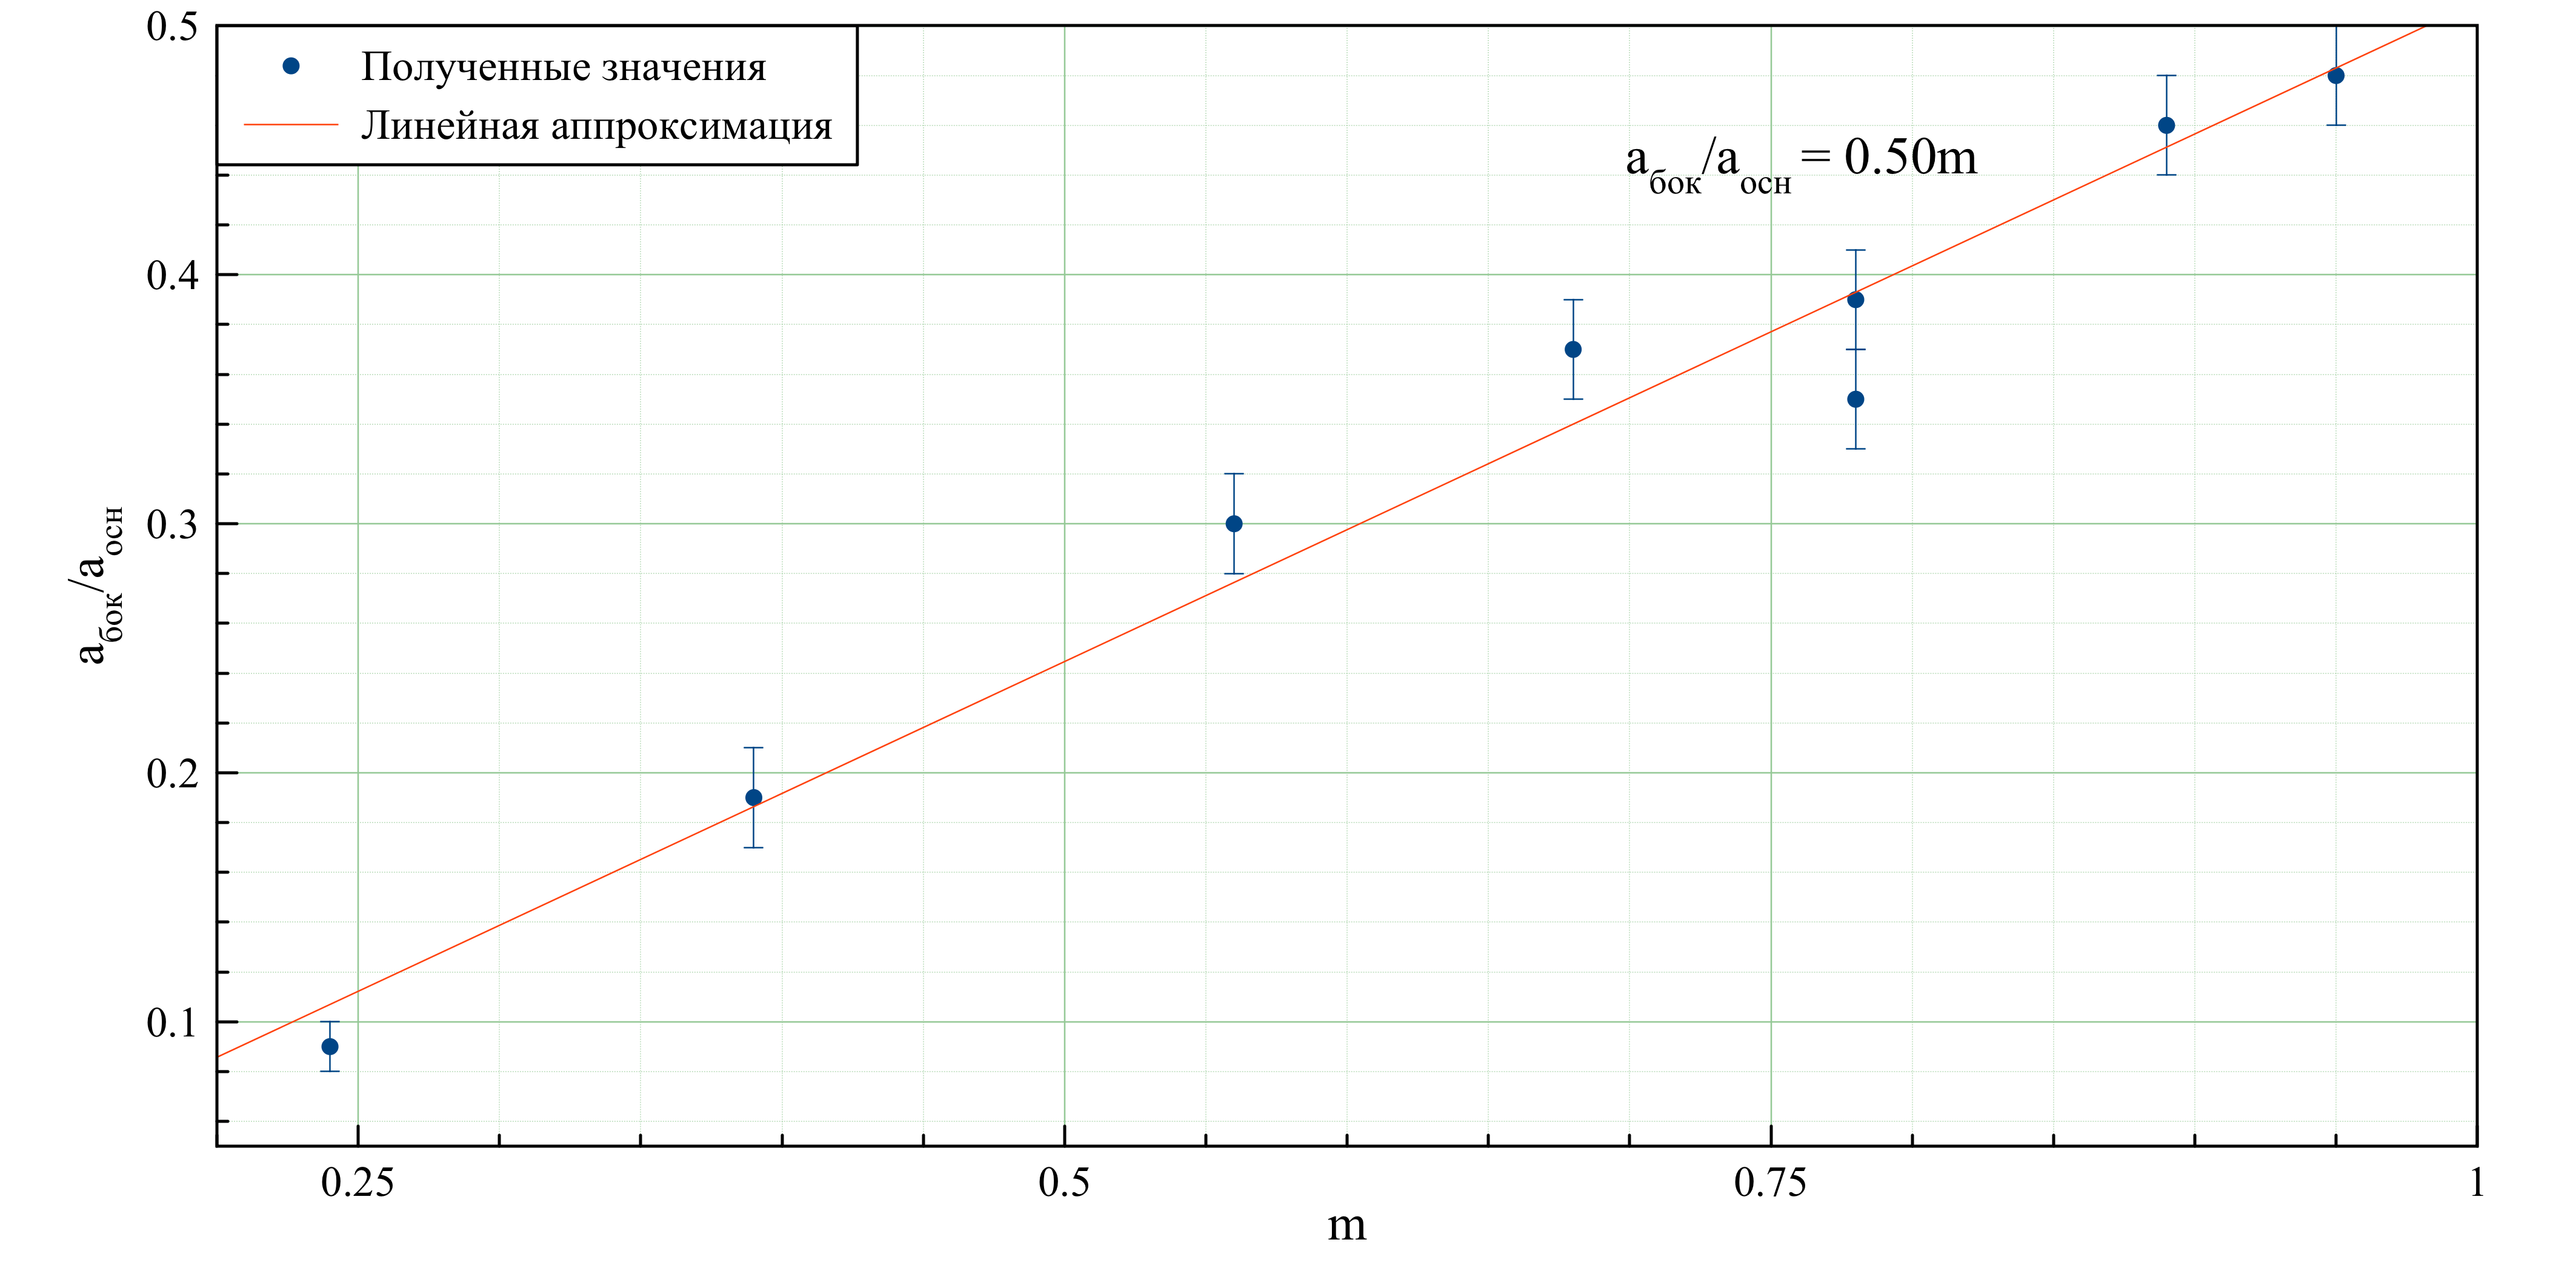
\includegraphics[width = \textwidth]{GraphC}
\caption{График зависимости $\dfrac{a_\text{бок}}{a_\text{осн}}(m)$}
\end{figure}

Коэффициент угла наклона прямой и его погрешность посчитаем методом наименьших квадратов: $k = \dfrac{\langle \frac{a_\text{бок} m}{a_\text{осн}}  \rangle}{\langle m^2 \rangle}$, $\sigma_k = \dfrac{1}{\sqrt{n}} \sqrt{\dfrac{\langle \left( \frac{a_\text{бок}}{a_\text{осн}}\right)^2 \rangle}{\langle m^2 \rangle} - k^2}$, тогда $\dfrac{a_\text{бок}}{a_\text{осн} m} = 0.5 \pm 0.01$

\section{Вывод}

Экспериментально было проверено соотношение неопределенности в первых двух экспериментах. Точность достаточно высокая, полученные значения соответствуют ожиданиям. Основной вклад в погрешность вносит отсутствие мелких делений на анализаторе спектра.

В третьем эксперименте было проверена зависимость отношения амплитуд спектральных линий синусоидального сигнала, модулированного низкочастотными гармоническими колебаниями, от коэффициента модуляции.
\end{document}